% Copyright 2026 Sreeram Anil
% SPDX-License-Identifier: CC-BY-4.0
% =============================================================================
%  Second-order extended Kalman filter — classical Kalman family
% =============================================================================
\chapter{Second-Order Extended Kalman Filter (SO-EKF)}
\label{ch:soekf}

\section*{At a glance}
\begin{tabular}{@{}l>{\raggedright\arraybackslash}p{0.76\textwidth}@{}}
Family & classical Kalman \\
Header & \texttt{include/estkit/filters/soekf.hpp} \\
Registered name & \texttt{SO-EKF} \\
State dimension & $n_x = 4$ (cell model) --- generic in $n_x, n_u, n_y$ \\
Cost per step & $\mathcal{O}(n_x^4)$ traces, $2n_x(n_x{+}1)$ model calls per Hessian; $3.9$--$4.2\,\SI{}{\micro\second}$/step \\
Primary references & \cite{athans1968,jazwinski1970,bass1966,maybeck1982vol2,gelb1974} \\
\end{tabular}

\section{Motivation and aerospace/BMS relevance}
The EKF truncates the Taylor expansion of $f$ and $h$ after the linear term. The next term is
not small when the state uncertainty is large: for a scalar function $\phi$ and
$\vx\sim\N{\xhat}{\mP}$,
\begin{equation}
\E{\phi(\vx)} = \phi(\xhat) + \tfrac12\tr\!\left(\nabla^2\phi(\xhat)\,\mP\right) + \mathcal{O}(\mP^2),
\label{eq:soekf-motivation}
\end{equation}
so the EKF's predicted measurement is biased by $\tfrac12\tr(\nabla^2h\,\mP)$ and its
innovation covariance is too small by a term of the same order squared. Athans, Wishner and
Bertolini~\cite{athans1968} derived the filter that keeps these terms --- the ``modified
truncated second-order filter'' --- and demonstrated on a scalar nonlinear example that it
removes a bias the EKF cannot see. Jazwinski~\cite[Ch.~9]{jazwinski1970} and
Bass, Norum and Schwartz~\cite{bass1966} give the general Gaussian second-order form.

For SOC estimation this term has a concrete meaning: it is the curvature of the OCV
characteristic. When $\sigma_\soc$ is at its start-up value of $0.1$, the average of
$\ocv(\soc)$ over the prior differs from $\ocv(\hat{\soc})$ by tens of millivolts --- more
than ten times the voltage-sensor noise --- and the true variance of the predicted voltage is
substantially larger than $\mH\mP\mH^\T+\mR$. An EKF that ignores both becomes confident too
early and locks in whatever error it made on the first update. This chapter shows that
correcting it explicitly is the single most effective change made to the EKF in this family.

\section{Problem statement and assumptions}
Model \eqref{eq:ekf-proc}--\eqref{eq:ekf-meas}. $f$ and $h$ are assumed twice continuously
differentiable, and the conditional density is assumed Gaussian so that the third central
moment vanishes and the fourth factorises (Isserlis' theorem) --- these are exactly the
assumptions that make the trace formulae below exact to the stated order. Write
$\nabla^2 f_i$ and $\nabla^2 h_i$ for the $n_x\times n_x$ Hessians of the $i$-th components
of $f$ and $h$.

\section{Derivation}
\paragraph{Mean correction.} Expanding $f_i$ to second order about $\xplus_{k-1}$ with
$\bm{e} = \vx - \xplus_{k-1}$, $\E{\bm e}=\bm0$, $\E{\bm e\bm e^\T}=\Pplus_{k-1}$:
\begin{equation}
\E{f_i(\vx)} = f_i(\xplus_{k-1}) + \underbrace{\E{\nabla f_i^\T\bm e}}_{=0}
 + \tfrac12\E{\bm e^\T\nabla^2f_i\,\bm e} + \dots
 = f_i(\xplus_{k-1}) + \tfrac12\tr\!\left(\nabla^2f_i\,\Pplus_{k-1}\right) + \dots
\label{eq:soekf-mean}
\end{equation}
using $\E{\bm e^\T\mA\bm e} = \tr(\mA\,\E{\bm e\bm e^\T})$.

\paragraph{Covariance correction.} For the $(i,j)$ entry, keeping terms up to second order in
$\mP$ and using the Gaussian fourth-moment identity
$\E{\bm e^\T\mA\bm e\,\bm e^\T\mB\bm e} = \tr(\mA\mP)\tr(\mB\mP) + 2\tr(\mA\mP\mB\mP)$,
\begin{equation}
\left(\operatorname{Cov}[f(\vx)]\right)_{ij}
= \left(\mF\mP\mF^\T\right)_{ij} + \tfrac12\tr\!\left(\nabla^2f_i\,\mP\,\nabla^2f_j\,\mP\right) + \dots
\label{eq:soekf-cov}
\end{equation}
(the $\tr(\mA\mP)\tr(\mB\mP)$ part is cancelled exactly by the mean correction
\eqref{eq:soekf-mean}, which is why the mean and covariance corrections must be applied
together). The same two formulae applied to $h$ give the corrected predicted measurement and
innovation covariance. Collecting:
\begin{align}
\xminus_k &= f(\xplus_{k-1},\vu_{k-1}) + \tfrac12\sum_i \bm{e}_i\,\tr\!\left(\nabla^2f_i\,\Pplus_{k-1}\right),
\label{eq:soekf-tu-mean}\\
\Pminus_k &= \mF\Pplus_{k-1}\mF^\T + \mQ
 + \tfrac12\left[\tr\!\left(\nabla^2f_i\,\Pplus_{k-1}\nabla^2f_j\,\Pplus_{k-1}\right)\right]_{ij},
\label{eq:soekf-tu-cov}\\
\yhat_k &= h(\xminus_k,\vu_k) + \tfrac12\sum_i \bm{e}_i\,\tr\!\left(\nabla^2h_i\,\Pminus_k\right),
\label{eq:soekf-ymean}\\
\tilde{\mR}_k &= \mR + \tfrac12\left[\tr\!\left(\nabla^2h_i\,\Pminus_k\nabla^2h_j\,\Pminus_k\right)\right]_{ij},
\qquad \mS_k = \mH\Pminus_k\mH^\T + \tilde{\mR}_k,
\label{eq:soekf-S}
\end{align}
with $\bm e_i$ the $i$-th unit vector. The gain and the state update are the EKF's,
$\mK_k = \Pminus_k\mH^\T\mS_k\inv$, $\xplus_k = \xminus_k + \mK_k(\vy_k-\yhat_k)$.

\begin{proposition}[Joseph form remains exact]\label{prop:soekf-joseph}
With $\mK_k = \Pminus_k\mH^\T\mS_k\inv$ and $\mS_k$ as in \eqref{eq:soekf-S},
\begin{equation}
(\mI-\mK_k\mH)\Pminus_k(\mI-\mK_k\mH)^\T + \mK_k\tilde{\mR}_k\mK_k^\T
= \Pminus_k - \mK_k\mS_k\mK_k^\T .
\label{eq:soekf-joseph}
\end{equation}
\end{proposition}
\begin{proof}
Expanding the left side gives
$\Pminus - \mK\mH\Pminus - \Pminus\mH^\T\mK^\T + \mK(\mH\Pminus\mH^\T+\tilde{\mR})\mK^\T
= \Pminus - \mK\mH\Pminus - \Pminus\mH^\T\mK^\T + \mK\mS\mK^\T$. Since
$\mK\mS\mK^\T = \Pminus\mH^\T\mS\inv\mH\Pminus = \mK\mH\Pminus = \Pminus\mH^\T\mK^\T$, this
equals $\Pminus - \mK\mS\mK^\T$.
\end{proof}
Proposition~\ref{prop:soekf-joseph} means the numerically preferable Joseph form can be used
unchanged provided $\mR$ is replaced by the inflated $\tilde{\mR}$ --- a point that is easy to
get wrong in implementations.

\paragraph{Numerical Hessians.} The model concept exposes $f$, $h$ and (optionally) their
Jacobians, never second derivatives, so the Hessians are built by central differences:
\begin{equation}
\left(\nabla^2 g_c\right)_{ab} \approx
\frac{g_c(\vx{+}h_a\bm e_a{+}h_b\bm e_b) - g_c(\vx{+}h_a\bm e_a{-}h_b\bm e_b)
 - g_c(\vx{-}h_a\bm e_a{+}h_b\bm e_b) + g_c(\vx{-}h_a\bm e_a{-}h_b\bm e_b)}{4h_ah_b},
\label{eq:soekf-hess}
\end{equation}
with $h_a = \rho(1+\abs{x_a})$. For $a=b$ this degenerates to the usual
$[g(\vx{+}2h)-2g(\vx)+g(\vx{-}2h)]/(4h^2)$. One sweep produces all $n_y$ (or $n_x$) component
Hessians simultaneously, costing $2n_x(n_x{+}1) = 40$ evaluations of the model for $n_x = 4$.

\section{Algorithm}
\begin{algorithm}[H]
\caption{SO-EKF --- one sampling period}
\begin{algorithmic}[1]
\Require $\xplus_{k-1},\Pplus_{k-1},\vu_{k-1},\vy_k,\vu_k$, Hessian step $\rho$
\State \textbf{Time update:} $\mF\gets\partial f/\partial\vx$;\;
       $\{\nabla^2f_i\}\gets$ central differences \eqref{eq:soekf-hess}
\State $\xminus_k\gets f(\xplus_{k-1},\vu_{k-1})+\tfrac12\sum_i\bm e_i\tr(\nabla^2f_i\Pplus_{k-1})$
\State $\Pminus_k\gets\mF\Pplus_{k-1}\mF^\T+\mQ+\tfrac12[\tr(\nabla^2f_i\Pplus\nabla^2f_j\Pplus)]_{ij}$; symmetrise
\State \textbf{Predicted measurement:} $\{\nabla^2h_i\}\gets$ central differences at $\xminus_k$ (cached)
\State $\yhat_k\gets h(\xminus_k,\vu_k)+\tfrac12\sum_i\bm e_i\tr(\nabla^2h_i\Pminus_k)$
\State \textbf{Measurement update:}
       $\tilde{\mR}\gets\mR+\tfrac12[\tr(\nabla^2h_i\Pminus\nabla^2h_j\Pminus)]_{ij}$;\;
       $\mS\gets\mH\Pminus_k\mH^\T+\tilde{\mR}$
\State $\mK\gets\Pminus_k\mH^\T\mS\inv$;\; $\xplus_k\gets\xminus_k+\mK(\vy_k-\yhat_k)$
\State $\Pplus_k\gets(\mI-\mK\mH)\Pminus_k(\mI-\mK\mH)^\T+\mK\tilde{\mR}\mK^\T$; symmetrise
\State \textbf{if} constraints enabled \textbf{then} $\xplus_k\gets\Pi(\xplus_k)$
\Ensure $\xplus_k,\Pplus_k$
\end{algorithmic}
\end{algorithm}

\section{Application to the battery model}
The cell dynamics are affine in $\vx$, so $\nabla^2 f_i \equiv \bm0$ and the entire
second-order content sits in the measurement equation, where the only non-zero Hessian entry
is $\partial^2\ocv/\partial\soc^2$ (the $\mH$ entries for $v_1,v_2,h$ are constants). The
mean correction is therefore
\begin{equation}
\yhat_k = h(\xminus_k,\vu_k) + \tfrac12\,\ocv''(\soc)\,\sigma_\soc^2,
\qquad
\tilde{R} = R + \tfrac12\left(\ocv''(\soc)\,\sigma_\soc^2\right)^2 ,
\label{eq:soekf-battery}
\end{equation}
which at start-up ($\sigma_\soc = 0.1$, $\ocv''\approx -6$\,V) is a $-30$\,mV bias correction
and adds $1.8\times10^{-3}$\,V$^2$ to an innovation variance of $5.6\times10^{-3}$\,V$^2$
(a $32\,\%$ inflation, against a sensor term $\mR = 4.4\times10^{-6}$\,V$^2$ that is four
hundred times smaller), and in steady state
($\sigma_\soc\approx10^{-3}$) is $3\,\SI{}{\micro\volt}$ and nothing. The filter therefore
degrades gracefully to the EKF exactly when the EKF is right.

\paragraph{Choice of the differencing step.} This is the one real implementation decision.
The theoretically optimal relative step for a second derivative in double precision is
$\varepsilon^{1/4}\approx 1.2\times10^{-4}$, which balances round-off against truncation for a
\emph{smooth} function. The estimator-side OCV, however, is a $241$-point piecewise-linear
table with spacing $0.005$ in SOC: its exact second derivative is zero inside a segment and a
delta at the knots, so a stencil narrower than the table spacing returns either $0$ or a
spike, and the correction becomes a noise source instead of a bias correction. The stencil
must span several segments. With $h_a = \rho(1+\abs{\soc})\approx 2\rho$ and a half-width of
$2h_a$, requiring at least eight segments gives
$4\rho \gtrsim 8\times0.005 \Rightarrow \rho\gtrsim 10^{-2}$; requiring the stencil to stay
well inside the scale on which the OCV curve itself varies ($\approx 0.1$ SOC) gives
$\rho\lesssim 2\times10^{-2}$. The default \code{hess\_step = }$10^{-2}$ follows from the
table geometry, not from the benchmark data.

The measurement is direct: sweeping $\rho$ over $\{10^{-4},10^{-3},3{\times}10^{-3},10^{-2},
3{\times}10^{-2},10^{-1}\}$ gives, on \texttt{combined}
($\text{RMSE}/\text{RMSE}_{\text{ss}}$ in per cent SOC, one seed):
$17.2/13.8$ (i.e.\ the plain EKF --- the correction is invisible), $0.66/0.42$, $1.23/1.57$,
$0.56/0.68$, $17.7/14.8$, $15.3/11.5$. The useful window $10^{-3}\le\rho\le10^{-2}$ is exactly
the one predicted by the table geometry, and the collapse at both ends is exactly the expected
round-off / truncation failure. The sensitivity \emph{within} the window (a factor of two on
\texttt{combined}) is a genuine caveat and is discussed below; it also explains why the
three-seed mean at the default $\rho = 10^{-2}$, $1.00/1.28\,\%$, is a little above the
single-seed value quoted here.

Options: \code{hess\_step} $=10^{-2}$, \code{hessian\_f = true}, \code{hessian\_h = true},
\code{second\_order\_cov = true}, \code{joseph = true}, \code{apply\_constraints = true}.

\section{Implementation notes}
\code{kalman\_detail::numeric\_hessian} is a small template that fills an array of $M$
component Hessians from one $\mathcal{O}(n_x^2)$ stencil sweep. The measurement Hessian is
cached together with the $(\vx,\vu)$ at which it was computed, because the benchmark adapter
calls \code{predict\_measurement(u)} and then \code{update(y,u)} with the same arguments ---
without the cache the filter would pay for the sweep twice. The cost breakdown per step is
$40$ evaluations of $f$ (all of which return zero Hessians on this model and can be disabled
with \code{hessian\_f = false} for a $2\times$ speed-up), $40$ of $h$, and
$n_x^2 + n_y^2$ trace terms; measured $3.9$--$4.2\,\SI{}{\micro\second}$, the second most
expensive filter in the family after the GHKF. \code{sizeof(SecondOrderEkf<EcmModel>)} is
4496\,bytes.

In single precision the differencing amplifies round-off by $1/(4h_ah_b)\approx 600$, giving a
Hessian noise floor of $\approx 3\times10^{-4}$ against a signal of $\approx 6$; the float
build costs a visible factor of two on the easiest scenario
($\text{RMSE}_{\text{ss}} = 0.07\,\%$ on \texttt{nominal} in float against $0.03\,\%$ in
double, the largest nominal float penalty of the EKF family) while improving the hard ones
($1.45\,\%$ against $1.79\,\%$ on \texttt{aged\_cell}); with analytic Hessians the penalty
disappears.

\section{Benchmark results}
% Copyright 2026 Sreeram Anil
% SPDX-License-Identifier: CC-BY-4.0
\begin{table}[H]\centering\footnotesize\setlength{\tabcolsep}{4pt}
\caption{SO-EKF: cell-level benchmark on the eVTOL mission (mean over seeds; RMSE and max error in \% SOC; $t_\mathrm{conv}$: first time the error stays below 2\,\% for 60\,s, -- = never; EKF reference: steady-state RMSE of the plain EKF on the same data).}\label{tab:cell_SOEKF}
\begin{tabular}{llrrrrrcrr}\toprule
plant & scenario & RMSE & RMSE$_\mathrm{ss}$ & max & $t_\mathrm{conv}$ [s] & RMSE$_v$ [mV] & div. & EKF ref. & ns/step \\ \midrule
ECM & nominal & 0.26 & 0.04 & 3.95 & 0 & 1.04 & no & 0.05 & 4202 \\
ECM & init\_error & 0.13 & 0.08 & 3.09 & 0 & 2.05 & no & 0.05 & 4196 \\
ECM & current\_bias & 0.61 & 0.62 & 3.74 & 0 & 1.08 & no & 0.61 & 4200 \\
ECM & noise\_step & 0.29 & 0.14 & 3.95 & 0 & 2.97 & no & 0.12 & 4196 \\
ECM & outliers & 0.64 & 0.30 & 4.22 & 74 & 2.19 & no & 0.21 & 4197 \\
ECM & cold & 0.34 & 0.13 & 3.94 & 0 & 2.01 & no & 0.16 & 4211 \\
ECM & hot & 0.19 & 0.03 & 3.97 & 0 & 0.87 & no & 0.03 & 4195 \\
ECM & aged\_cell & 1.22 & 1.56 & 4.34 & 0 & 3.87 & no & 1.52 & 4191 \\
ECM & param\_mismatch & 0.77 & 0.89 & 4.24 & 0 & 2.89 & no & 1.36 & 4198 \\
ECM & sensor\_dropout & 0.36 & 0.18 & 3.95 & 0 & 1.85 & no & 0.46 & 4189 \\
ECM & preisach & 1.52 & 0.20 & 5.58 & 226 & 1.16 & no & 0.20 & 4215 \\
ECM & combined & 1.00 & 1.28 & 7.44 & 0 & 4.64 & no & 12.44 & 4232 \\
\midrule
SPM & nominal & 3.44 & 3.52 & 4.52 & 0 & 1.26 & no & 3.73 & 3961 \\
SPM & init\_error & 4.12 & 4.13 & 5.00 & -- & 2.10 & no & 3.81 & 3970 \\
SPM & current\_bias & 4.82 & 5.58 & 6.27 & 0 & 1.33 & no & 5.69 & 3964 \\
SPM & noise\_step & 3.26 & 3.19 & 4.52 & 0 & 3.23 & no & 3.30 & 3992 \\
SPM & outliers & 1.23 & 1.27 & 8.18 & 0 & 2.53 & no & 1.99 & 3955 \\
SPM & cold & 8.12 & 8.16 & 10.42 & -- & 4.62 & no & 7.35 & 3957 \\
SPM & hot & 2.07 & 2.13 & 4.41 & 0 & 1.00 & no & 2.16 & 3932 \\
SPM & param\_mismatch & 3.93 & 4.14 & 4.85 & 0 & 2.10 & no & 3.13 & 3923 \\
SPM & sensor\_dropout & 4.97 & 5.13 & 5.65 & 0 & 2.09 & no & 5.31 & 3960 \\
\bottomrule\end{tabular}\end{table}

\begin{figure}[H]\centering
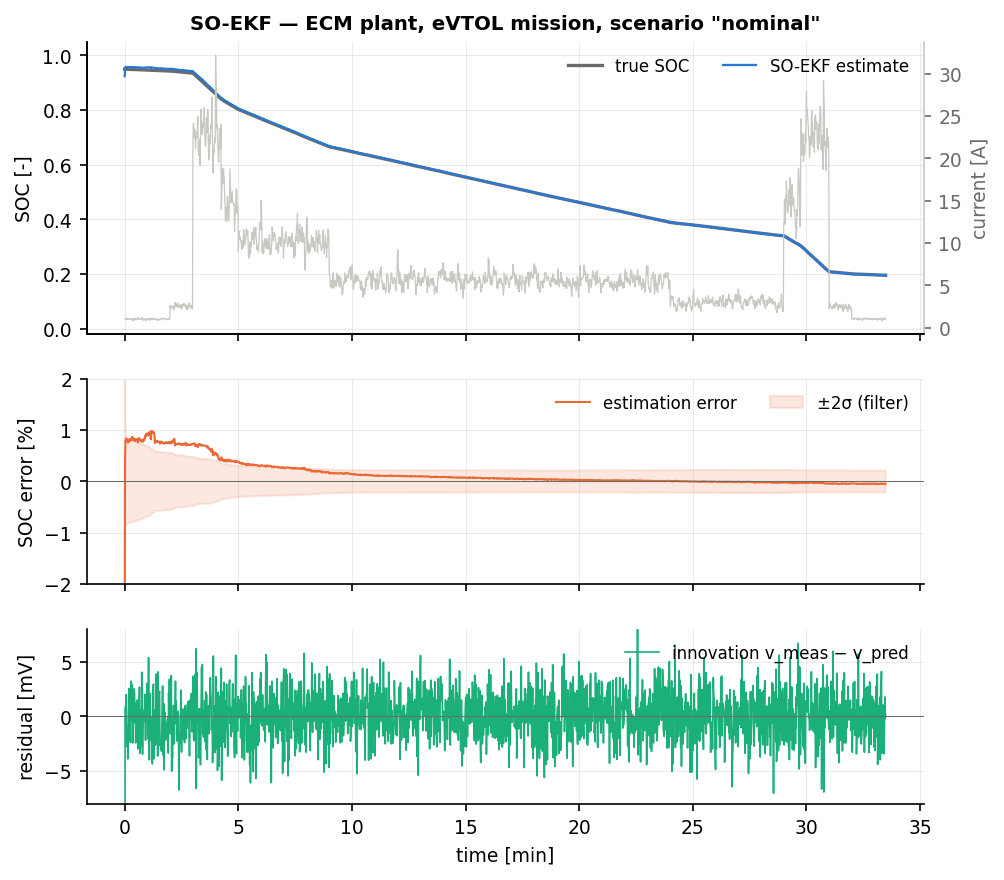
\includegraphics[width=\textwidth]{figures/cell_SOEKF_nominal.png}
\caption{SO-EKF on the nominal eVTOL mission: true and estimated SOC (top), estimation error with the $\pm 2\sigma$ band when available (middle), voltage residual (bottom).}
\end{figure}
\begin{figure}[H]\centering
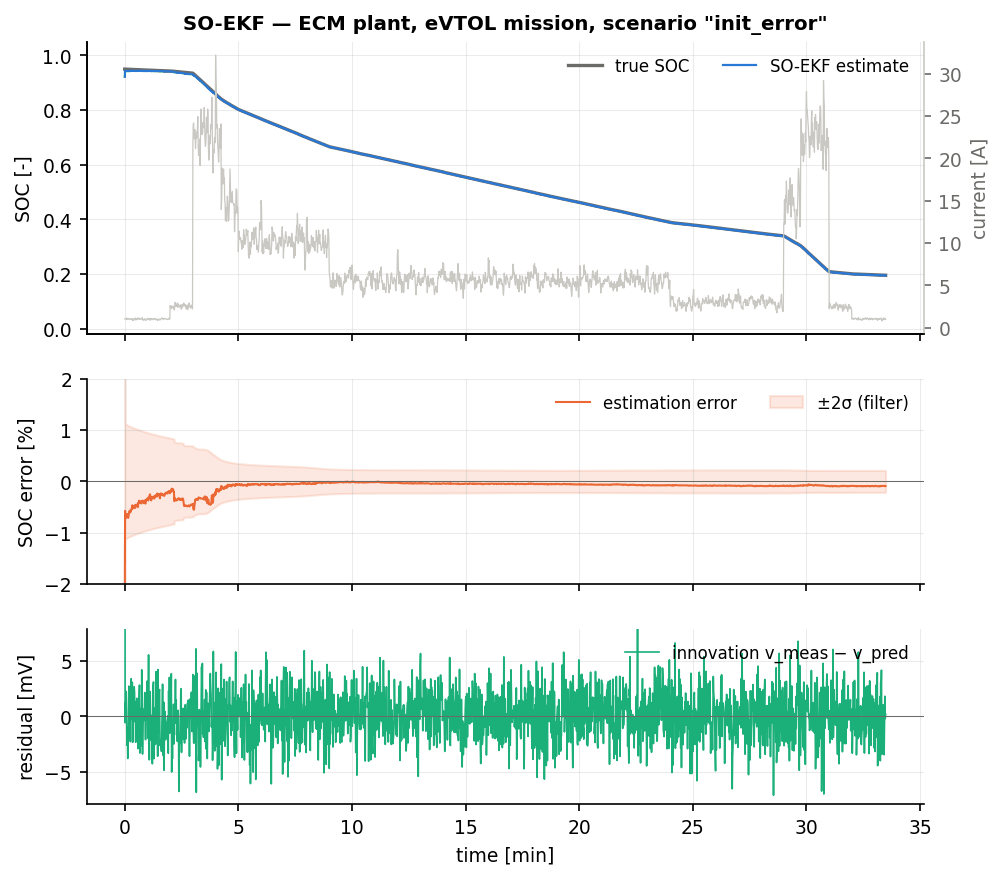
\includegraphics[width=\textwidth]{figures/cell_SOEKF_init_error.png}
\caption{SO-EKF with a 35\,\% initial SOC error.}
\end{figure}
\begin{figure}[H]\centering
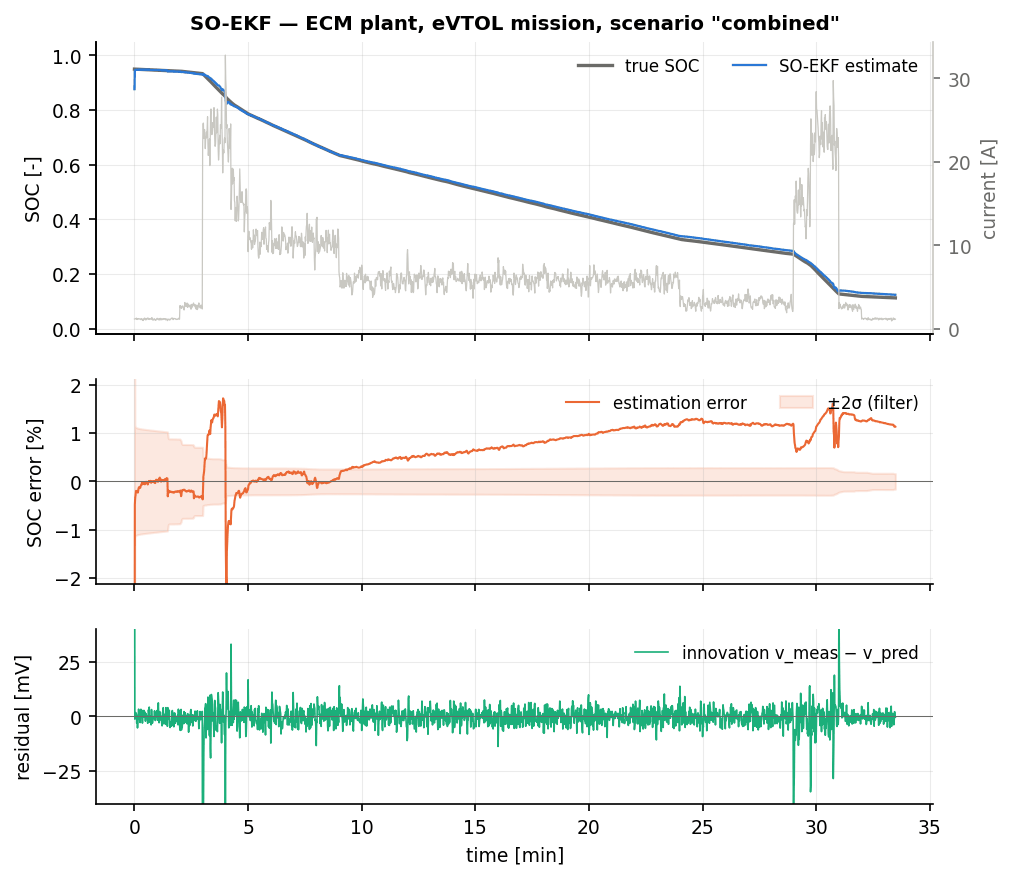
\includegraphics[width=\textwidth]{figures/cell_SOEKF_combined.png}
\caption{SO-EKF on the \texttt{combined} scenario: the explicit curvature term inflates $\tilde{\mR}$, the posterior variance does not collapse, and the filter finds the true SOC before the high-current segment.}
\end{figure}

All numbers are three-seed means in per cent SOC.

The SO-EKF is one of the three effective repairs of the EKF in this family. On
\texttt{combined} --- the scenario the EKF, CKF, CKF5, CDKF, GHKF, EIF, SR-EKF and UD-EKF all
fail --- it reaches $\text{RMSE} = 1.00\,\%$, $\text{RMSE}_{\text{ss}} = 1.28\,\%$ and
converges in the first sample, against the EKF's $16.02/12.44\,\%$ and never. It is
essentially tied with the UKF ($1.19\,\%$) and ahead of the IPLF ($1.72\,\%$) and the IEKF
($2.13\,\%$); the earlier development run, on a single seed, made the SO-EKF look twice as good
as the UKF, and the three-seed means show that the two are within their scatter of each other.
The mechanism is exactly \eqref{eq:soekf-battery}: at $k = 0$ the inflated $\tilde{R}$ prevents
the posterior variance from collapsing, the filter stays open to correction for the next few
seconds, and it finds the true SOC before the high-current segment begins.

It also gives the equal-best steady-state nominal accuracy of the family
($\text{RMSE}_{\text{ss}} = 0.04\,\%$, tied with the UKF and SR-UKF), the best
\texttt{sensor\_dropout} result of the fifteen ($0.36/0.18\,\%$ against the EKF's
$0.72/0.46\,\%$ --- the same inflation prevents the stuck voltage from being trusted), and a
large improvement on \texttt{param\_mismatch} ($0.77/0.89\,\%$ against $1.28/1.36\,\%$, second
only to the IPLF).

The cost appears in the whole-run metrics on easy scenarios: \texttt{nominal} RMSE $0.26\,\%$
against the EKF's $0.15\,\%$ and a maximum error of $3.95\,\%$ against $1.07\,\%$. All of this
is the deliberate caution of the first few seconds, when the second-order terms are large and
the filter correctly refuses to trust a measurement equation it knows is a poor affine model.
\texttt{outliers} degrades to $0.30\,\%$ steady state (EKF $0.21\,\%$) and \texttt{aged\_cell}
to $1.56\,\%$ (EKF $1.52\,\%$), the latter for the same reason as the IPLF: with a persistently
biased model, a filter that keeps its gain alive longer tracks the bias further.
\texttt{preisach} deserves a note: its steady-state error, $0.20\,\%$, is exactly the EKF's,
but its whole-run RMSE of $1.52\,\%$ is the worst of the family and its convergence time
($226$\,s) the longest, because the inflated $\tilde{\mR}$ makes it slow to take up the
hysteresis offset at the start of the mission.

The honest caveat is the step-size sensitivity documented above: within the physically
justified window $10^{-3}\le\rho\le10^{-2}$ the \texttt{combined} result varies by a factor of
two, so the headline $1.28\,\%$ should be read as ``order $1\,\%$, an order of magnitude better
than the EKF'', not as a precise figure. A model that supplied analytic Hessians --- trivial
here, since $\ocv''$ is available in closed form from the Chen2020 fit --- would remove the
sensitivity entirely, and that is the recommended production route. The divided-difference
filter of Chapter~\ref{ch:cdkf} offers the alternative: its second difference is taken over
$\pm\sqrt3\sigma$, i.e. a stencil that scales itself with the covariance and never needs a
step-size choice at all. The float-versus-double table shows the other side of the same coin:
the SO-EKF's nominal steady-state error rises from $0.03\,\%$ in double to $0.07\,\%$ in
single precision, the largest relative degradation of the EKF-family filters, because the
differencing amplifies round-off by $1/(4h_ah_b)\approx600$.

\paragraph{SPM plant: structured model error.}
\begin{figure}[H]\centering
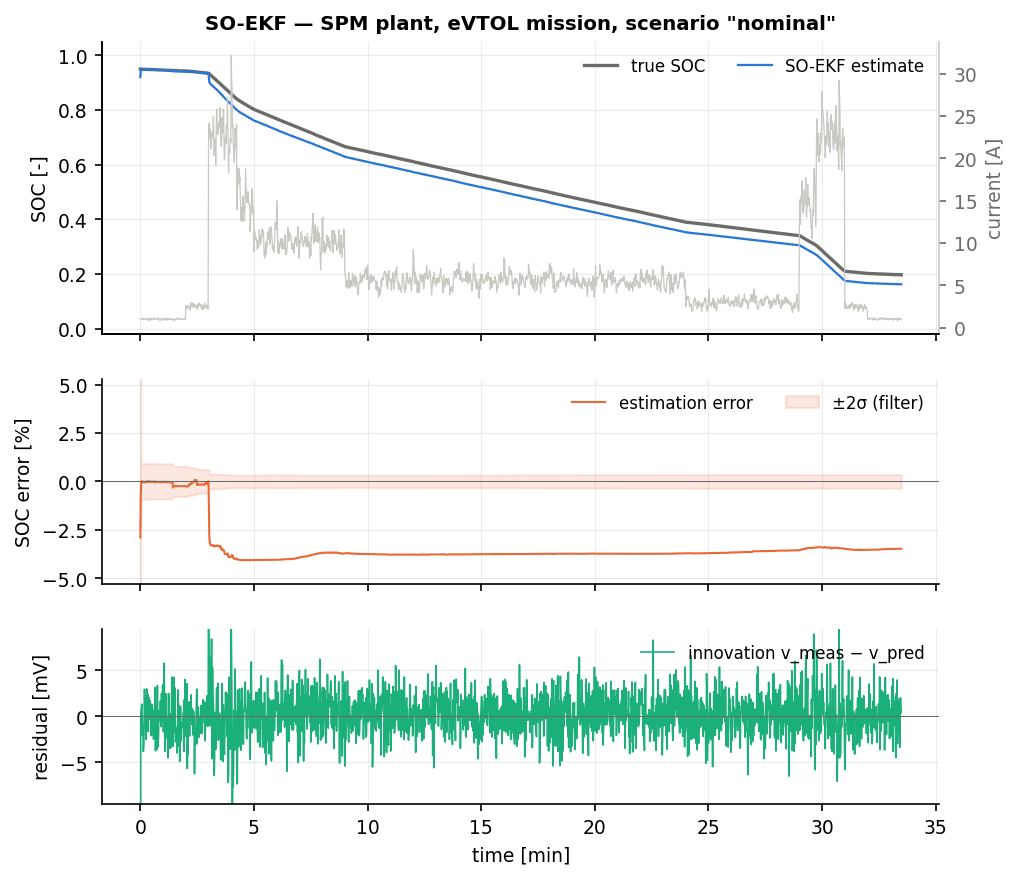
\includegraphics[width=\textwidth]{figures/cellspm_SOEKF_nominal.png}
\caption{SO-EKF on the nominal mission with the electrochemical (SPM) plant.}
\end{figure}
The SPM block of the table is a different kind of test. The plant is the electrochemical
single-particle model; the estimator still runs a 2-RC equivalent circuit, fitted to that plant,
which leaves a \emph{structured} residual of about $4$\,mV (Butler--Volmer kinetics and
solid-phase diffusion that no 2-RC circuit can reproduce) and a slow second branch,
$\tau_2 = 556$\,s. Over a $33$-minute mission a $556$\,s pole barely relaxes, so $v_2(t)$ is
close to an affine ramp --- and so is $\ocv(\soc(t))$ while the cell discharges at a roughly
constant rate. The two channels through which the measurement sees the state,
$(\partial\ocv/\partial\soc)\,\delta\soc$ and $-\delta v_2$, are therefore nearly collinear in
the information accumulated over the flight: the pair $(\soc, v_2)$ is close to unobservable,
and no filter can decide whether a persistent few-millivolt residual belongs to the slow RC
branch or to the state of charge. Because that direction is weakly observable, a $4$\,mV
structured error maps onto \emph{several per cent} of SOC instead of the
$4\,\text{mV}/0.8\,\text{V}\approx0.5\,\%$ a well-conditioned channel would give. This
$(\soc,v_2)$ ambiguity, not the size of the residual, is the mechanism behind the
$3.7$--$4.6\,\%$ band in which the whole classical family sits.

The SO-EKF is the best of the Jacobian-based filters on the SPM plant apart from the LKF:
$3.52\,\%$ on \texttt{nominal} against the EKF's $3.73\,\%$, $1.27\,\%$ on \texttt{outliers}
against $1.99\,\%$ (the best SPM outlier result of the family), $5.13\,\%$ on
\texttt{sensor\_dropout} against $5.31\,\%$ and $5.58\,\%$ on \texttt{current\_bias} against
$5.69\,\%$. The reason is the same inflation that wins \texttt{combined}: adding
$\tfrac12\tr(\nabla^2h\,\mP\,\nabla^2h\,\mP)$ to $\mR$ de-weights the OCV channel exactly when
$\sigma_\soc$ is large, which is precisely when the $(\soc,v_2)$ ambiguity is dangerous. The
effect is modest --- it does not lift the filter out of the band --- and it reverses on the two
rows where the prior stays wide for a long time: \texttt{cold} $8.16\,\%$ against the EKF's
$7.35\,\%$ and \texttt{param\_mismatch} $4.14\,\%$ against $3.13\,\%$. A curvature correction
addresses nonlinearity; the SPM residual is not curvature, it is a missing state.

\section{Summary}
The Gaussian second-order EKF adds two terms to the EKF: a bias correction
$\tfrac12\tr(\nabla^2h\,\mP)$ on the predicted measurement and an inflation
$\tfrac12\tr(\nabla^2h\,\mP\,\nabla^2h\,\mP)$ of the innovation covariance. On this benchmark
those two terms turn the EKF's worst failure into a result on a par with the UKF's, deliver the
equal-best steady-state nominal accuracy and the best \texttt{sensor\_dropout} result of all
fifteen filters, and cost about nine times an EKF step when the Hessians are computed
numerically (much less with analytic ones). Use it when the measurement function has
significant curvature over the prior --- which for an OCV-based SOC estimator is the case at
every cold start. Do not use a fixed finite-difference step on a look-up-table model without
checking the stencil against the table spacing, expect a visible penalty in single precision,
and remember that the second-order term helps with nonlinearity, not with model error: on the
SPM plant it gains $6\,\%$ relative to the EKF, not a factor.
